% ============================================================
%  TurkLang 2026 — Conference presentation
%  Paper: A Gold-Standard Dependency Treebank for the Uzbek Language
%  Authors: S. Matlatipov, M. Kurbanova
%  Target length: 13 minutes
%  Theme: LDV Beamer (provided in ./ldvtheme)
% ============================================================
\documentclass[10pt,aspectratio=169]{beamer}
\mode<presentation>{\usetheme{ldv}\setbeamercovered{transparent}}

\usepackage[utf8]{inputenc}
\usepackage[T1]{fontenc}
\usepackage{lmodern}
\usepackage{amsmath,amssymb}
\usepackage{graphicx}
\usepackage{booktabs}
\usepackage{array}
\usepackage{tabularx}   % required by the LDV outer theme (header bar)
\usepackage{colortbl}   % required by the LDV theme
\usepackage{xcolor}
\usepackage{tikz}
\usepackage{tikz-dependency}
\usetikzlibrary{positioning,arrows.meta,shapes,fit,backgrounds}

% ---- Highlight colour shortcuts for tikz-dependency ----
\definecolor{hlgreen}{RGB}{60,150,75}
\definecolor{hlblue}{RGB}{0,101,189}    % LDV blue
\definecolor{hlorange}{RGB}{227,114,34} % LDV orange
\definecolor{hlred}{RGB}{200,40,40}

\depstyle{hl-edge}{edge style={hlorange, ultra thick}, label style={fill=hlorange!20,draw=hlorange}}
\depstyle{hl-blue}{edge style={hlblue,  ultra thick}, label style={fill=hlblue!15, draw=hlblue}}
\depstyle{hl-green}{edge style={hlgreen, ultra thick}, label style={fill=hlgreen!15,draw=hlgreen}}

% ---- LDV theme header strings ----
\newcommand{\slidenomenclature}{Slide}
\newcommand{\zwischentitel}{TurkLang 2026}
\newcommand{\leitthema}{Matlatipov \& Kurbanova}

% ---- Titlepage ----
\title{A Gold-Standard Dependency Treebank\\for the Uzbek Language}
\subtitle{XIV International Conference on Computer Processing of Turkic Languages\\\textbf{TurkLang 2026}}
\author{Sanatbek Matlatipov \and Mukhabbat Kurbanova}
\newcommand{\presdatum}{2026}
\institute{National University of Uzbekistan\\Tashkent, Uzbekistan}

\begin{document}

% ====== 1. Title ======
\begin{frame}[plain]
   \titlepage
   \begin{tikzpicture}[remember picture, overlay]
     % Top-left: ENU logo
     \node[anchor=north west, inner sep=8pt]
       at (current page.north west)
       {
\includegraphics[height=1.2cm]{images/enu}};
     % Top-right: IEEE Siberia logo
     \node[anchor=north east, inner sep=8pt]
       at (current page.north east)
       {
\includegraphics[height=1.2cm]{images/IEEE_siberia}};
     % Bottom-right: combined universities logo
     \node[anchor=south east, inner sep=10pt]
       at (current page.south east)
       {
\includegraphics[height=1.4cm]{images/universities}};
   \end{tikzpicture}
\end{frame}

% ====== 2. Outline ======
\begin{frame}{Outline}
   \begin{columns}[T,onlytextwidth]
     \begin{column}{0.5\textwidth}
       \begin{enumerate}
         \item Motivation \& related work
         \item Data collection
         \item Annotation workflow
         \item An annotated Uzbek sentence
         \item Inter-annotator agreement
       \end{enumerate}
     \end{column}
     \begin{column}{0.5\textwidth}
       \begin{enumerate}\setcounter{enumi}{5}
         \item Treebank statistics
         \item Linguistic profile
         \item Parsing experiments
         \item Results \& error analysis
         \item Conclusion \& future work
       \end{enumerate}
     \end{column}
   \end{columns}
   \vfill
   \small Focus today: the \textbf{resource} and its \textbf{evaluation} — not parser internals.
\end{frame}

% ====== 3. Motivation ======
\section{Motivation}
\begin{frame}{Why a new Uzbek treebank?}
   \begin{columns}[T,onlytextwidth]
     \begin{column}{0.58\textwidth}
       \begin{itemize}
         \item Uzbek: \textbf{Turkic}, agglutinative, SOV; $\sim$35M speakers.
         \item Rich nominal/verbal morphology — \emph{many} features per token.
         \item Until now: only \textbf{one} UD treebank (Uzbek-UT, 500 sentences, news+fiction).
         \item Parsing scores plateaued; coverage was narrow.
       \end{itemize}
       \vspace{0.4em}
       \begin{block}{Research question}
         Does a larger, multi-genre, double-annotated gold treebank meaningfully change parser performance for Uzbek?
       \end{block}
     \end{column}
     \begin{column}{0.4\textwidth}
       \centering
       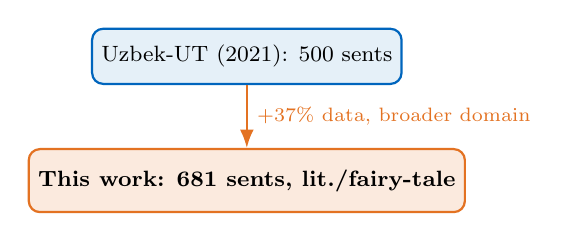
\begin{tikzpicture}[every node/.style={font=\footnotesize}]
         \node[draw=hlblue,thick,rounded corners,fill=hlblue!10,minimum width=3.2cm,minimum height=0.7cm] (a) {Uzbek-UT (2021): 500 sents};
         \node[draw=hlorange,thick,rounded corners,fill=hlorange!15,minimum width=3.6cm,minimum height=0.8cm,below=0.8cm of a] (b) {\textbf{This work: 681 sents, lit./fairy-tale}};
         \draw[-{Latex},thick,hlorange] (a) -- node[right,font=\scriptsize]{+37\% data, broader domain} (b);
       \end{tikzpicture}
     \end{column}
   \end{columns}
\end{frame}

% ====== 4. Related work ======
\begin{frame}{Where this fits in Uzbek NLP}
   \begin{itemize}
     \item \textbf{Treebanks:} Uzbek-UT (Akhundjanova \& Talamo, 2021) — first UD treebank, 500 sents.
     \item \textbf{Morphology:} Prolog-based analyser (Matlatipov, 2009); rule-based UzbekTagger (Sharipov et al.); recent analysers by Salaev et al., Abdurakhmonova et al.
     \item \textbf{Tasks:} sentiment / ABSA (Matlatipov et al., 2024).
   \end{itemize}
   \vspace{0.4em}
   \begin{alertblock}{Gap}
     No \emph{independent}, multi-domain, \emph{double-annotated} gold treebank with published IAA.
   \end{alertblock}
\end{frame}

% ====== 5. Contributions ======
\begin{frame}{Contributions}
   \begin{enumerate}
     \item A new \textbf{gold-standard Uzbek UD treebank}: 681 sentences, $\sim$7{,}950 tokens, $\sim$4{,}800 unique word forms.
     \item Annotation by \textbf{six annotators} (4 linguists + 2 NLP engineers) in INCEpTION; full double annotation + adjudication.
     \item Reported \textbf{inter-annotator agreement} (Cohen's $\kappa$, Krippendorff's $\alpha$).
     \item Comparative evaluation of \textbf{UDPipe, Stanza, spaCy} — \textbf{+3 to +7.5 LAS} over Uzbek-UT.
     \item Public release of the treebank in CoNLL-U.
   \end{enumerate}
\end{frame}

% ====== 6. Data collection ======
\section{Data}
\begin{frame}{Data sources}
   \begin{columns}[T,onlytextwidth]
     \begin{column}{0.55\textwidth}
       \begin{itemize}
         \item Fiction: \emph{Maqar}.
         \item Educational/literary: \emph{Kun shundan boshlanadi}.
         \item Publicly available \textbf{fairy tales}.
       \end{itemize}
       \vspace{0.5em}
       \begin{itemize}
         \item All in \textbf{Latin script}.
         \item Mean length $\approx$ \textbf{12 tokens}.
         \item \textbf{481 train / 200 test} ($\approx$ 29\% test).
       \end{itemize}
     \end{column}
     \begin{column}{0.42\textwidth}
       \centering
       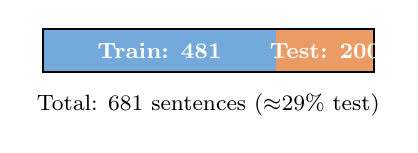
\begin{tikzpicture}[every node/.style={font=\footnotesize}]
         % Stacked bar: 481 train / 200 test of 681 sentences
         \def\W{4.2}     % total width in cm
         \def\TR{2.965}  % 481/681 * W
         \fill[hlblue!55]   (0,0) rectangle (\TR,0.55);
         \fill[hlorange!70] (\TR,0) rectangle (\W,0.55);
         \draw[thick] (0,0) rectangle (\W,0.55);
         \node[white] at (\TR/2,0.275) {\textbf{Train: 481}};
         \node[white] at ({(\TR+\W)/2},0.275) {\textbf{Test: 200}};
         \node[below=0.15cm] at (\W/2,0) {Total: 681 sentences ($\approx$29\% test)};
       \end{tikzpicture}
     \end{column}
   \end{columns}
\end{frame}

% ====== 7. Annotation workflow ======
\section{Annotation}
\begin{frame}{Annotation workflow}
   \begin{columns}[T,onlytextwidth]
     \begin{column}{0.55\textwidth}
       \begin{enumerate}
         \item Pre-tokenization (UD v2 rules).
         \item Pilot training on a shared seed set.
         \item \textbf{Double independent annotation} in INCEpTION.
         \item Disagreement adjudication \\(majority vote $\rightarrow$ senior linguist).
         \item Export to \textbf{CoNLL-U}.
       \end{enumerate}
       \vspace{0.3em}
       \footnotesize \textbf{Uzbek-specific decisions}
       \begin{itemize}
         \item Case suffixes $\rightarrow$ \texttt{Case=Acc}, \texttt{Case=Dat}, \ldots
         \item Postpositions: separate tokens, \texttt{case} relation.
         \item Null copula: \emph{no} explicit \texttt{cop} node.
       \end{itemize}
     \end{column}
     \begin{column}{0.43\textwidth}
       \centering
       % filename contains a space; brace it so LaTeX parses it correctly
       \IfFileExists{../Turklang_Gold_Treebank_fina/annatation progress.png}{%
         
\includegraphics[width=\linewidth]{{../Turklang_Gold_Treebank_fina/annatation progress}.png}%
       }{%
         \fbox{\parbox{0.9\linewidth}{\centering\footnotesize Annotation workflow figure\\(reused from the paper)}}%
       }\\[-0.2em]
       \scriptsize Six annotators: 4 linguists + 2 NLP engineers.
     \end{column}
   \end{columns}
\end{frame}

% ====== 8. Annotated example — TikZ dependency tree (real CoNLL-U: s2) ======
\begin{frame}{An annotated Uzbek sentence (\texttt{sent\_id = s2})}
   \centering
   \vspace{-0.2em}
   % \resizebox scales the tikzpicture to exactly the slide text width
   \resizebox{\linewidth}{!}{%
   \begin{dependency}[theme = simple, label style={font=\scriptsize}, edge slant=4pt]
      \begin{deptext}[column sep=0.20cm, row sep=0.12cm]
         Shu \& paytgacha \& bizda \& shevalar \& bo'yicha \& tadqiqotlarda \& ularning \& adabiy \& tildan \& farqi \& qancha \& ko'p \& ko'rsatilsa \& {,} \& shuncha \& ijobiy \& baholanib \& kelinmoqda \& {.} \\
         {\tiny PRON} \& {\tiny NOUN} \& {\tiny PRON} \& {\tiny NOUN} \& {\tiny ADP} \& {\tiny NOUN} \& {\tiny PRON} \& {\tiny ADJ} \& {\tiny NOUN} \& {\tiny NOUN} \& {\tiny PRON} \& {\tiny ADV} \& {\tiny VERB} \& {\tiny PUNCT} \& {\tiny PRON} \& {\tiny ADJ} \& {\tiny VERB} \& {\tiny VERB} \& {\tiny PUNCT} \\
      \end{deptext}
      % --- highlighted edges (the ones we discuss) ---
      \deproot[edge style={hlred,ultra thick},   label style={fill=hlred!15}]{17}{root}
      \depedge[edge style={hlorange,ultra thick},label style={fill=hlorange!20}]{17}{13}{advcl}
      \depedge[edge style={hlblue,ultra thick},  label style={fill=hlblue!15}]{13}{10}{nsubj}
      \depedge[edge style={hlgreen,ultra thick}, label style={fill=hlgreen!15}]{13}{3}{obl}
      \depedge[edge style={hlgreen,ultra thick}, label style={fill=hlgreen!15}]{13}{6}{obl}
      \depedge[edge style={hlblue,ultra thick},  label style={fill=hlblue!15}]{6}{4}{nmod}
      \depedge[edge style={hlblue,ultra thick},  label style={fill=hlblue!15}]{4}{5}{case}
      % remaining edges (lighter)
      \depedge[edge style={black!45}]{2}{1}{det}
      \depedge[edge style={black!45}]{13}{2}{advcl}
      \depedge[edge style={black!45}]{10}{7}{nmod}
      \depedge[edge style={black!45}]{9}{8}{amod}
      \depedge[edge style={black!45}]{10}{9}{iobj}
      \depedge[edge style={black!45}]{12}{11}{det}
      \depedge[edge style={black!45}]{13}{12}{advmod}
      \depedge[edge style={black!45}]{13}{14}{punct}
      \depedge[edge style={black!45}]{16}{15}{det}
      \depedge[edge style={black!45}]{17}{16}{advmod}
      \depedge[edge style={black!45}]{17}{18}{advcl}
      \depedge[edge style={black!45}]{18}{19}{punct}
   \end{dependency}%
   }% end \resizebox

   \vspace{0.3em}
   {\footnotesize\itshape `Until now, in studies on dialects, the more differences from the
   literary language are shown, the more positively they are evaluated.'}

   \vspace{0.3em}
   \begin{columns}[T,onlytextwidth]\footnotesize
     \begin{column}{0.5\textwidth}
       \textcolor{hlblue}{\texttt{case}} — postposition \texttt{bo'yicha} as a
       separate token attached to \texttt{shevalar}.
     \end{column}
     \begin{column}{0.5\textwidth}
       \textcolor{hlorange}{\texttt{advcl}} — conditional \texttt{ko'rsatilsa} $\to$
       root \texttt{baholanib}; \textcolor{hlgreen}{\texttt{obl}} from locative \texttt{-da}.
     \end{column}
   \end{columns}
\end{frame}

% ====== 9. IAA ======
\begin{frame}{Inter-annotator agreement}
   \centering
   \begin{tabular}{lcc}
      \toprule
      \textbf{Annotation layer} & \textbf{Cohen's $\kappa$} & \textbf{Krippendorff's $\alpha$}\\
      \midrule
      Lemmatization              & \textbf{95.2\%} & 94.6\%\\
      POS tagging (UPOS)         & 93.7\%          & 94.1\%\\
      Morphological features     & 90.8\%          & 89.9\%\\
      \bottomrule
   \end{tabular}
   \vspace{0.8em}

   \begin{itemize}
      \item Computed across all 6 annotators on the doubly annotated pool.
      \item \textbf{Lemma + UPOS} above 93\% — strong agreement on closed layers.
      \item \textbf{Morphology} slightly lower — agglutinative ambiguity in derivational suffixes.
   \end{itemize}
\end{frame}

% ====== 10. Treebank statistics ======
\section{Corpus}
\begin{frame}{Treebank statistics vs.\ Uzbek-UT}
   \centering
   \begin{tabular}{lccc}
      \toprule
      \textbf{Treebank} & \textbf{Sentences} & \textbf{Tokens} & \textbf{Unique forms}\\
      \midrule
      \textbf{Lit./fairy-tale (ours)} & \textbf{681}  & \textbf{7{,}950} & \textbf{4{,}800}\\
      Uzbek-UT (news + fiction)       & 500           & 5{,}850          & 3{,}523\\
      \midrule
      Relative size                   & +36\%         & +36\%            & +36\%\\
      \bottomrule
   \end{tabular}
   \vspace{0.8em}

   \begin{itemize}
      \item $\approx$ 11.6 tokens / sentence.
      \item All \textbf{17 UD POS} categories covered.
      \item \textbf{45} morph-feature values (vs.\ 42 in Uzbek-UT).
      \item \textbf{34} dependency labels (vs.\ 32) — adds \texttt{discourse}, \texttt{parataxis}, \texttt{vocative}, \texttt{ccomp}.
   \end{itemize}
\end{frame}

% ====== 11. Linguistic profile ======
\begin{frame}{Linguistic profile}
   \begin{columns}[T,onlytextwidth]
     \begin{column}{0.5\textwidth}
       \textbf{POS distribution}
       \begin{itemize}\small
         \item NOUN $\sim$30\%, VERB $\sim$20\%, ADJ $\sim$15\%
         \item PROPN $\sim$8\% (vs.\ $\sim$5\% in Uzbek-UT)
         \item NUM $\sim$2.5\% (vs.\ $\sim$1.5\%) — educational content
       \end{itemize}
       \vspace{0.4em}
       \textbf{Morphology}
       \begin{itemize}\small
         \item $\sim$52\% of tokens carry features
         \item 6 cases; tense/mood on verbs; person+number agreement
       \end{itemize}
     \end{column}
     \begin{column}{0.5\textwidth}
       \textbf{Dependency relations (most frequent)}
       \begin{itemize}\small
         \item \texttt{nsubj} $\sim$12\%
         \item \texttt{case}  $\sim$9\%
         \item \texttt{obl}   $\sim$9\%
         \item \texttt{obj}   $\sim$8\%
       \end{itemize}
       \vspace{0.4em}
       \textbf{New constructions vs.\ Uzbek-UT}
       \begin{itemize}\small
         \item \texttt{vocative}, \texttt{ccomp}, \texttt{discourse} markers from literary / fairy-tale dialogue.
       \end{itemize}
     \end{column}
   \end{columns}
\end{frame}

% ====== 12. Experimental setup ======
\section{Experiments}
\begin{frame}{Experimental setup}
   \begin{itemize}
      \item Three widely-used UD parsers (treated as black boxes):
      \begin{itemize}
         \item \textbf{UDPipe} — classical pipeline baseline.
         \item \textbf{Stanza} — neural BiLSTM + character CNN.
         \item \textbf{spaCy}  — transition-based, tok2vec embeddings.
      \end{itemize}
      \item \textbf{Splits:}
      \begin{itemize}
         \item Ours: 481 train / 200 test.
         \item Uzbek-UT: 400 train / 100 test (genre-balanced).
      \end{itemize}
      \item Gold tokenization; default hyperparameters; same protocol on both treebanks.
      \item \textbf{Metrics:} LAS, UAS, UPOS.
   \end{itemize}
\end{frame}

% ====== 13. Results ======
\begin{frame}{Parsing results across both treebanks}
   \centering
   \begin{tabular}{lccc|ccc}
      \toprule
      \textbf{Parser} & \multicolumn{3}{c|}{\textbf{Uzbek-UT (Akhundjanova \& Talamo, 2021)}} & \multicolumn{3}{c}{\textbf{Lit./fairy-tale (this work)}}\\
      \cmidrule(lr){2-4}\cmidrule(lr){5-7}
                     & LAS  & UAS  & UPOS & LAS  & UAS  & UPOS\\
      \midrule
      UDPipe         & 52.0 & 55.5 & 93.0 & 55.0 & 63.0 & 94.5\\
      spaCy          & 60.0 & 62.5 & 94.0 & 61.0 & 69.0 & 96.0\\
      \textbf{Stanza}& \textbf{62.0} & \textbf{66.0} & \textbf{95.0} & \textbf{66.0} & \textbf{74.0} & \textbf{97.0}\\
      \bottomrule
   \end{tabular}
   \vspace{0.6em}

   \begin{itemize}\small
      \item \textbf{Same protocol, same parsers} — only the training treebank changes.
      \item Uzbek-UT remains a \textbf{strong foundation}: all three parsers already exceed 50 LAS on it.
      \item Our \textbf{literary/fairy-tale} treebank covers a different domain and adds double annotation, so the numbers are \textbf{complementary, not competitive}.
      \item \textbf{Stanza} leads on both — character-level features suit Uzbek's agglutinative morphology.
   \end{itemize}
\end{frame}

% ====== 13b. Training curves (Stanza on the combined treebanks) ======
\begin{frame}{How the Stanza parser learns Uzbek}
   \begin{columns}[T,onlytextwidth]
     \begin{column}{0.58\textwidth}
       \centering
       \IfFileExists{images/parser_dev_curve.png}{%
         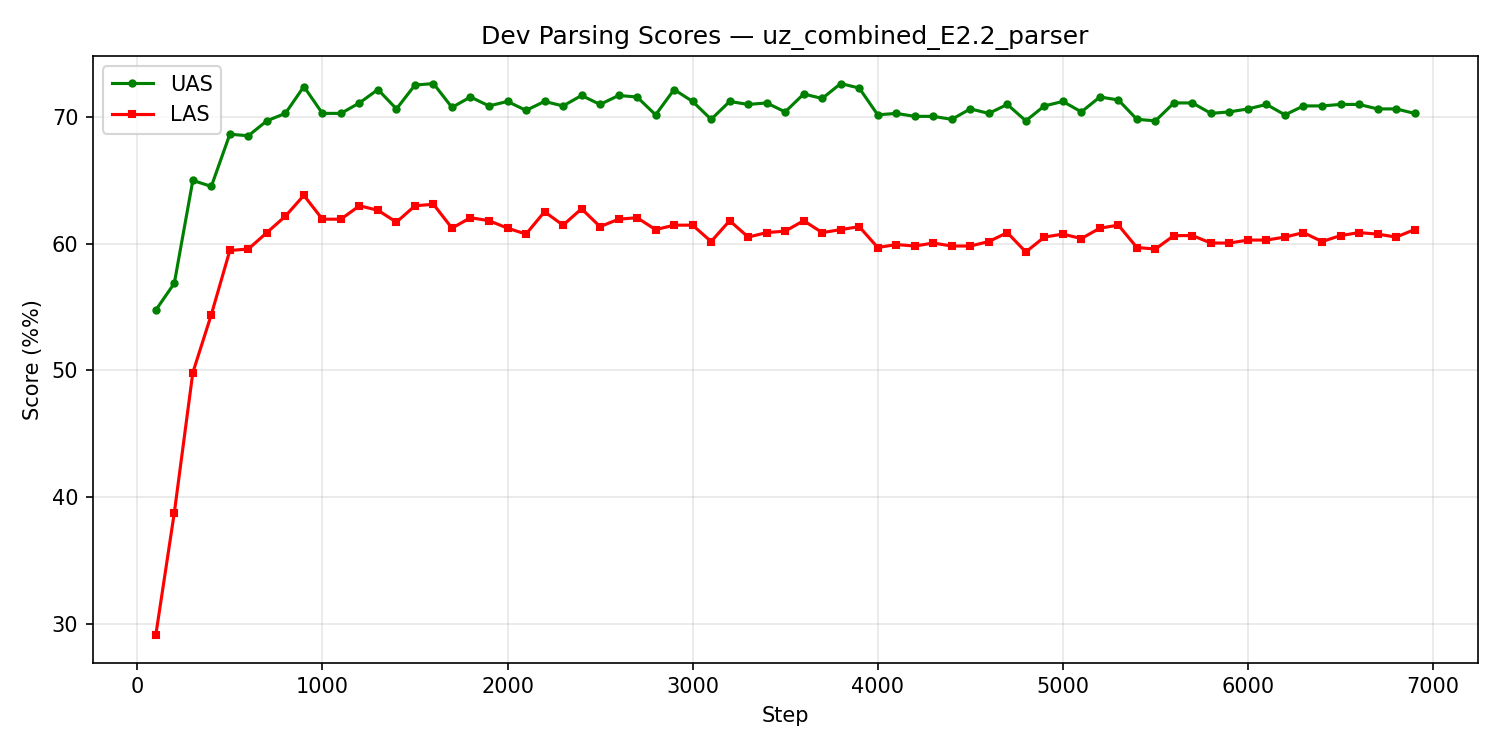
\includegraphics[width=\linewidth]{images/parser_dev_curve.png}%
       }{%
         \fbox{\parbox{0.9\linewidth}{\centering\footnotesize Stanza dev LAS/UAS curve}}%
       }\\[-0.1em]
       \scriptsize Dev UAS/LAS over training steps (Stanza parser, both treebanks merged).
     \end{column}
     \begin{column}{0.4\textwidth}\small
       \begin{itemize}
         \item UAS climbs to $\sim$72 and LAS to $\sim$63 within the first 1{,}000 steps.
         \item Both curves \textbf{plateau early} — the model is data-limited, not under-trained.
         \item Motivates our conclusion: \textbf{more annotated data} (across treebanks) is the most direct path to better Uzbek parsing.
       \end{itemize}
     \end{column}
   \end{columns}
\end{frame}

% ====== 14. Error analysis ======
\begin{frame}{Error analysis}
   \begin{columns}[T,onlytextwidth]
     \begin{column}{0.55\textwidth}
       Recurring confusions across all three parsers:
       \begin{itemize}
         \item \textbf{\texttt{advcl} boundaries} — subordinate clause attachment.
         \item \textbf{Coordination} attachment — long NP chains.
         \item \textbf{\texttt{nmod} vs.\ \texttt{obl}} — case-marked nominals.
       \end{itemize}
       Driver: Uzbek's \textbf{flexible word order} on top of SOV.\\[0.3em]
       Direction: contextual embeddings (e.g.\ multilingual BERT, XLM-R).
     \end{column}
     \begin{column}{0.43\textwidth}
       \centering
       \begin{dependency}[theme=simple, label style={font=\tiny}]
          \begin{deptext}[column sep=0.25cm]
              \ldots \& shevalar \& bo‘yicha \& tadqiqotlarda \& \ldots\\
          \end{deptext}
          \depedge[edge style={hlorange,thick}]{4}{2}{?nmod / ?obl}
          \depedge[edge style={hlblue,thick}]{2}{3}{case}
       \end{dependency}\\[-0.4em]
       \scriptsize Postposition + case-marked noun $\rightarrow$ ambiguous attachment.
     \end{column}
   \end{columns}
\end{frame}

% ====== 15. Conclusion ======
\section{Conclusion}
\begin{frame}{Conclusion}
   \begin{itemize}
      \item A new \textbf{gold-standard Uzbek UD treebank}: 681 sents, $\sim$8k tokens, double-annotated.
      \item \textbf{IAA} $\geq$ 90\% across all layers; $\geq$ 95\% on lemma.
      \item Consistent \textbf{LAS gains} for UDPipe, spaCy, Stanza over Uzbek-UT.
      \item Stanza reaches \textbf{66 LAS / 97 UPOS} — a real step up for Uzbek parsing.
   \end{itemize}
   \vspace{0.5em}
   \begin{block}{Future work}
      \begin{itemize}
         \item Extend to conversational, social-media, scholarly genres.
         \item Transformer-based parsers (mBERT, XLM-R, TURNA).
         \item Cross-lingual transfer with Turkish, Kazakh, Kyrgyz.
      \end{itemize}
   \end{block}
\end{frame}

% ====== 16. Thank you ======
\begin{frame}[plain]
   \begin{center}
      {\Large \textbf{Thank you!}}\\[0.6em]
      {\large Questions?}\\[1.2em]
      \begin{tabular}{rl}
         Contact: & \texttt{s.matlatipov@nuu.uz}\\
         Paper:   & \emph{A Gold-Standard Dependency Treebank for the Uzbek Language}\\
         Venue:   & TurkLang 2026\\
      \end{tabular}\\[1em]
      \footnotesize
      Thanks to E.~Kuriyozov (eval review), K.~Madinabonu \& M.~Shaydo (annotation),\\
      and R.~Hulkaroy (morphological feature guidelines).
   \end{center}
\end{frame}

\end{document}
